\documentclass[12pt,a4paper]{article}

\usepackage[utf8]{inputenc}
\usepackage[ngerman]{babel}
\usepackage[T1]{fontenc}
\usepackage{amsmath}
\usepackage{amsfonts}
\usepackage{amssymb}
\usepackage{graphicx}
\usepackage[left=2cm,right=2cm,top=2cm,bottom=2cm]{geometry}
\usepackage{multicol}
\usepackage{booktabs}
\usepackage[hidelinks]{hyperref}
\usepackage{tikz}
\usepackage{pgfplots}
\usepackage{blindtext}
\usepackage{array}
\usepackage{multirow}
\usepackage{bigdelim}
\usepackage{colortbl}
\usepackage{fancyhdr} 
\usepackage{tabularx}
\usepackage{xcolor}
\usepackage{color}
\usetikzlibrary{decorations.text}
\usetikzlibrary{tikzmark}
\pagestyle{fancy} 
	\fancyhf{} 
	\fancyhead[L]{
\includegraphics[scale=0.05]{Bilder/dhbw.png}} 
	\fancyhead[C]{\slshape Projektmanagement} 
	\fancyhead[R]{\slshape LaTeX Version}

\usepackage{helvet}
\renewcommand{\familydefault}{\sfdefault}

\author{\slshape Robin Rausch, Florian Maslowski, Ozan Akzebe}
\title{Projektmanagement}
\date{\slshape \today}
\begin{document}
\maketitle
\section{Fragenkatalog}
\begin{enumerate}
	\item Wie ist ein Projekt definiert (Eigenschaften)?
		\begin{enumerate}
		\item[] Einmaligkeit der Bedingungen 
		\item[] Zielvorgabe 
		\item[] Begrenzungen von Ressourcen (Zeit, Finanzen, Personal)
		\item[] Abgrenzung zu anderen Vorhaben 
		\item[] Projektspezifische Organisation 
		\end{enumerate}
	\item Was ist Projektmanagement?
		\begin{enumerate}
		\item[] Führungskonzept zur zielorientierten Durchführung großer Vorhaben 
		\item[] Gesamtheit der Führungsaufgaben 
			\begin{enumerate}
			\item[*] Zielsetzung
			\item[*] Planung
			\item[*] Steuerung
			\item[*] Überwachung
			\end{enumerate}
		\item[] Führungsaufbaus (Projektorganisation)
		\item[] Führungstechnik (Führungsstil) 
		\item[] Führungsmittel (Methoden) 
		\end{enumerate}
	\item Warum gehen Projekte schief?
		\begin{enumerate}
		\item[] Unklare Definition der Projektziele und Aufgaben 
		\item[] Falsche Einschätzung von Risiken 
		\item[] Verschiedene Projektvorstellungen die nicht abgestimmt werden  
		\item[] Ungenügende Kommunikation im Team 
		\end{enumerate}
	\item Was ist die Aufgabe eines Projektmanagers?
		\begin{enumerate}
		\item[] Aufgabenverteilung und Priorisierung 
		\item[] Kommunikation zwischen Gruppen 
		\item[] Ziele festlegen und erreichen  
		\item[] Konfliktbewältigung 
		\item[] Sicherstellung der Wirtschaftlichkeit  
		\item[] Entscheidung über Inhalt und Projektablauf 
		\end{enumerate}
	\item Welches sind die drei Säulen der PRM-Kompetenz?
		\begin{enumerate}
		\item[] Fachliche Kompetenz 
		\item[] Soziale Kompetenz
		\item[] Wirtschaftliche Kompetenz 
		\end{enumerate}
	\item Wozu dient das PM-BoK (Body of Knowledge)?
		\begin{enumerate}
		\item[] Kann Firmenspezifisch angewendet werden 
		\item[] Informationen über die Wissensgebiete im Projektmanagement  
			\begin{enumerate}
			\item[*] Integrationsmanagement
			\item[*] Umfangsmanagement
			\item[*] Terminmanagement
			\item[*] Kostenmanagement
			\item[*] Qualitätsmanagement
			\item[*] Personalmanagement
			\item[*] Kommunikationsmanagement
			\item[*] Risikomanagement
			\item[*] Beschaffungsmanagement
			\end{enumerate}
		\end{enumerate}
	\item Wozu benötigt man Ziele im Projekt und wie unterteilt man diese?
		\begin{enumerate}
		\item[] Um den Soll-Zustand festzustellen (Was soll erreicht werden?) 
		\item[] Unterteilung in: 
			\begin{enumerate}
			\item[*] Funktionale Ziele (Qualitative Ziele)
			\item[*] Operationale Ziele (Quantitative Ziele)
			\end{enumerate}
		\end{enumerate}
	\item An welches Prinzip sollten sich Ziele anlehnen?
		\begin{enumerate}
		\item[] SMART: 
			\begin{enumerate}
			\item[*] S: Spezifisch
			\item[*] M: Messbar
			\item[*] A: Angemessen
			\item[*] R: Realistisch
			\item[*] T: Terminierbar
			\end{enumerate}
		\end{enumerate}
	\item Welche Ziele dienen zur Messung des Erfolgs eines Projekts?
		\begin{enumerate}
		\item[] Sachziele
		\item[] Terminziele
		\item[] Kostenziele
		\end{enumerate}
	\item Was versteht man unter dem magischen Dreieck im PRM?
		\begin{enumerate}
		\item[] Zirkuläre Abhängigkeiten
		\item[] \includegraphics[scale=0.3]{Bilder/magischesDreieck.PNG}
		\end{enumerate}
	\item Was ist ein Zielsystem?
		\begin{enumerate}
		\item[] Ein Oberziel wird in mehrere Ziele unterteilt
		\end{enumerate}
	\item Verschiedene Projektorganisationen
	\begin{enumerate}
		\item[] Einfluß Projektmanagement
		\item[] 
		\item[] Matrix Projektmanagement
		\item[] 
		\item[] Reines Projektmanagement
		\begin{enumerate}
			\item[] 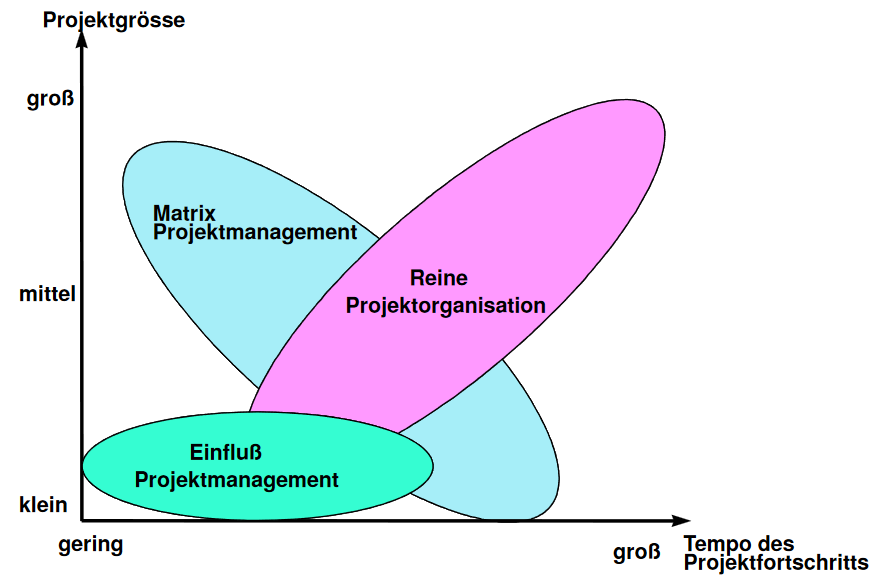
\includegraphics[scale=0.6]{Bilder/projektorganisationenWirksamkeit.PNG}
		\end{enumerate}
	\end{enumerate}
	\item Warum gibt es in der Analysephase eine solch große Begriffsvielfalt an Dokumenten?
	\begin{enumerate}
		\item Es gibt keine internationale Normung und somit viele verschiedene Begriffe und vorallem auch viele Synonyme.
	\end{enumerate}
	\item Was unterscheidet in der Projektphase das Lasten- vom Pflichtenheft?
	\begin{enumerate}
		\item Das Lastenheft wird zuerst erstellt und beeinhaltet nur die Forderungen des Auftraggebers, während das Pflichtenheft auf dem Lastenheft aufbaut und deutlich spezifischer ist. Das Pflichtenheft dient als Vertrags- und Einigungsgrundlage.
	\end{enumerate}
	\item Was beschreibt das Lastenheft und wer erstellt es?
	\begin{enumerate}
		\item Das Lastenheft beschreibt die Anforderungen an das Projekt und wird vom Auftraggeber erstellt.
	\end{enumerate}
	\item Was beschreibt das Pflichtenheft und wer erstellt es?
	\begin{enumerate}
		\item Das Pflichtenheft beinhaltet die detallierte Umsetzung des Projektes und wird vom Auftragnehmer(Projektleiter) erstellt.
	\end{enumerate}
	\item Wozu dient der Projektplan(Projektakte) und was enthält er?
	\begin{enumerate}
		\item Kostenplan
		\item Zeitplan
		\item Risikoplan
		\item ...
	\end{enumerate}
	\item Was versteht man unter einem Projekttagebuch und was enthält es?
	\begin{enumerate}
		\item Ablauf und Übersicht vom Projekt und dient zur Übersicht
	\end{enumerate}
	\item Was ist ein Projektstrukturplan und wozu wird er verwendet?
	\begin{enumerate}
		\item Darstellung der Teilprojekte und ? 
		\item Dient zur Übersicht
	\end{enumerate}
	\item Warum und wie strukturieren wir Projekte?
	\begin{enumerate}
		\item Zusammenhänge aufdecken und verstehen
		\item Übersichtlichkeit mithilfe von Baumstruktur
	\end{enumerate}
	\item Nach welchem Vorgehen werden Projekte strukturiert und wie entscheide ich mich für eine Methode?
	\begin{enumerate}
		\item Top-Down oder Bottom-Up
		\item Entscheidung abhängig davon, wie viel Erfahrung vorhanden ist und ob die Ziele klar definiert sind
	\end{enumerate}
	\item Wie detalliert strukturieren wir Projekte?
	\begin{enumerate}
		\item So detalliert wie notwendig.
		\item Bis zu einer bestimmten zeitlichen Ebene
	\end{enumerate}
	\item Wie sind AP's definiert und auf welcher Ebene des PSP's sind diese zu finden?
	\begin{enumerate}
		\item Unterste Ebene des PSP's
		\item Beinhalten Kostenschätzung, Zeitschätzung, \dots
		\item Hat Verantwortlichkeiten
	\end{enumerate}
	\item Was ist beim Schätzen von Aufwendungen wichtig?
	\begin{enumerate}
		\item Je mehr Wissen und Erfahrung, desto besser bzw. genauer wird die Schätzung
	\end{enumerate}
	\item Welche Schätzmethoden kennen sie und erklären sie diese?
	\begin{enumerate}
		\item Planning Poker
		\begin{enumerate}
			\item Team schätzt unabhängig von einander eine Task
			\item Wahl zwischen verschieden Fibonacci-Zahlen
			\item Team muss einstimmig wählen
			\item Bei unterschiedlichen Schätzungen wird sich drüber unterhalten und erneut geschätzt
		\end{enumerate}
		\item Dreipunkt-Methode
		\begin{enumerate}
			\item optimistische Schätzung
			\item mittlere Schätzung
			\item pessimistische Schätzung
		\end{enumerate}
	\end{enumerate}
	\item Wann ist ein Projekt wirtschaftlich?
	\begin{enumerate}
		\item Wenn der Gewinn höher ist als die Kosten
	\end{enumerate}
	\item Was versteht man unter einem kritischen Pfad?
	\begin{enumerate}
		\item Der Pfad, der am wenigsten Puffer hat und somit die größte Aufmerksamkeit benötigt. Dieser Pfad bestimmt oft die Länge/Dauer des Projektes.
	\end{enumerate}
	\item Welches sind die 4 Einflussgrößen für die Berechnung des Aufwandes eines Projektes?
	\begin{enumerate}
		\item Qualität
		\item Quantität
		\item Anzahl Mitarbeiter
		\item Produktivität
		\item \textcolor{red}{Dauer? --> Fehler: Eins muss raus... sind 5}
	\end{enumerate}
	\item Wie erstellt man einen Zeitplan für ein Projekt?
	\begin{enumerate}
		\item Gedanken machen über Aufgaben, ihre Dauer, ihren Anfangstermin und ihre Reihenfolge
	\end{enumerate}
	\newpage
	\item Was ist ein Gantt-Diagramm?
	\begin{enumerate}
		\item Aktivitäten in zeitlichen Balken
	\end{enumerate}
	\begin{center}
		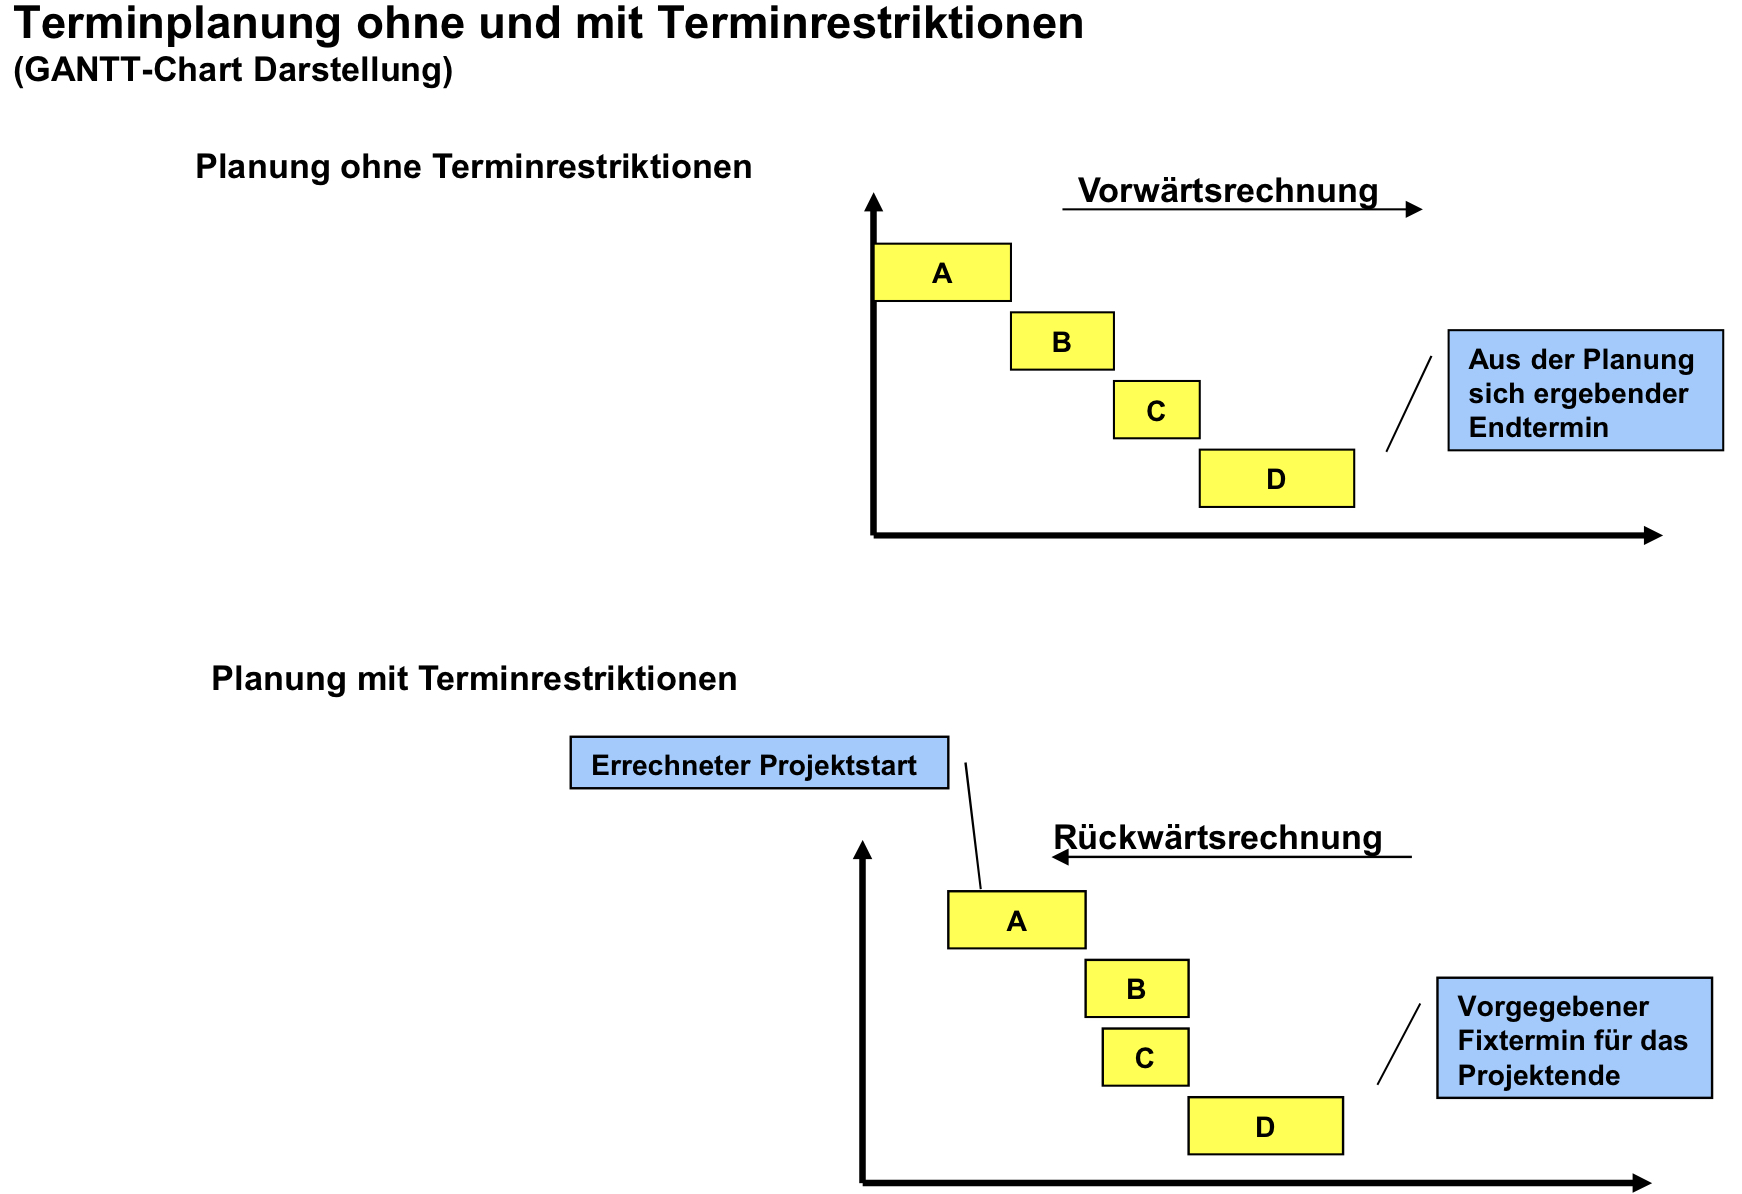
\includegraphics[scale=.175]{Bilder/Gantt.JPG}	
	\end{center}
	\item Was ist der MPM-Netzplan und wie ist dessen Darstellung?
	\begin{enumerate}
		\item Projektablauf als Graph dargestellt
	\end{enumerate}
	\begin{center}
		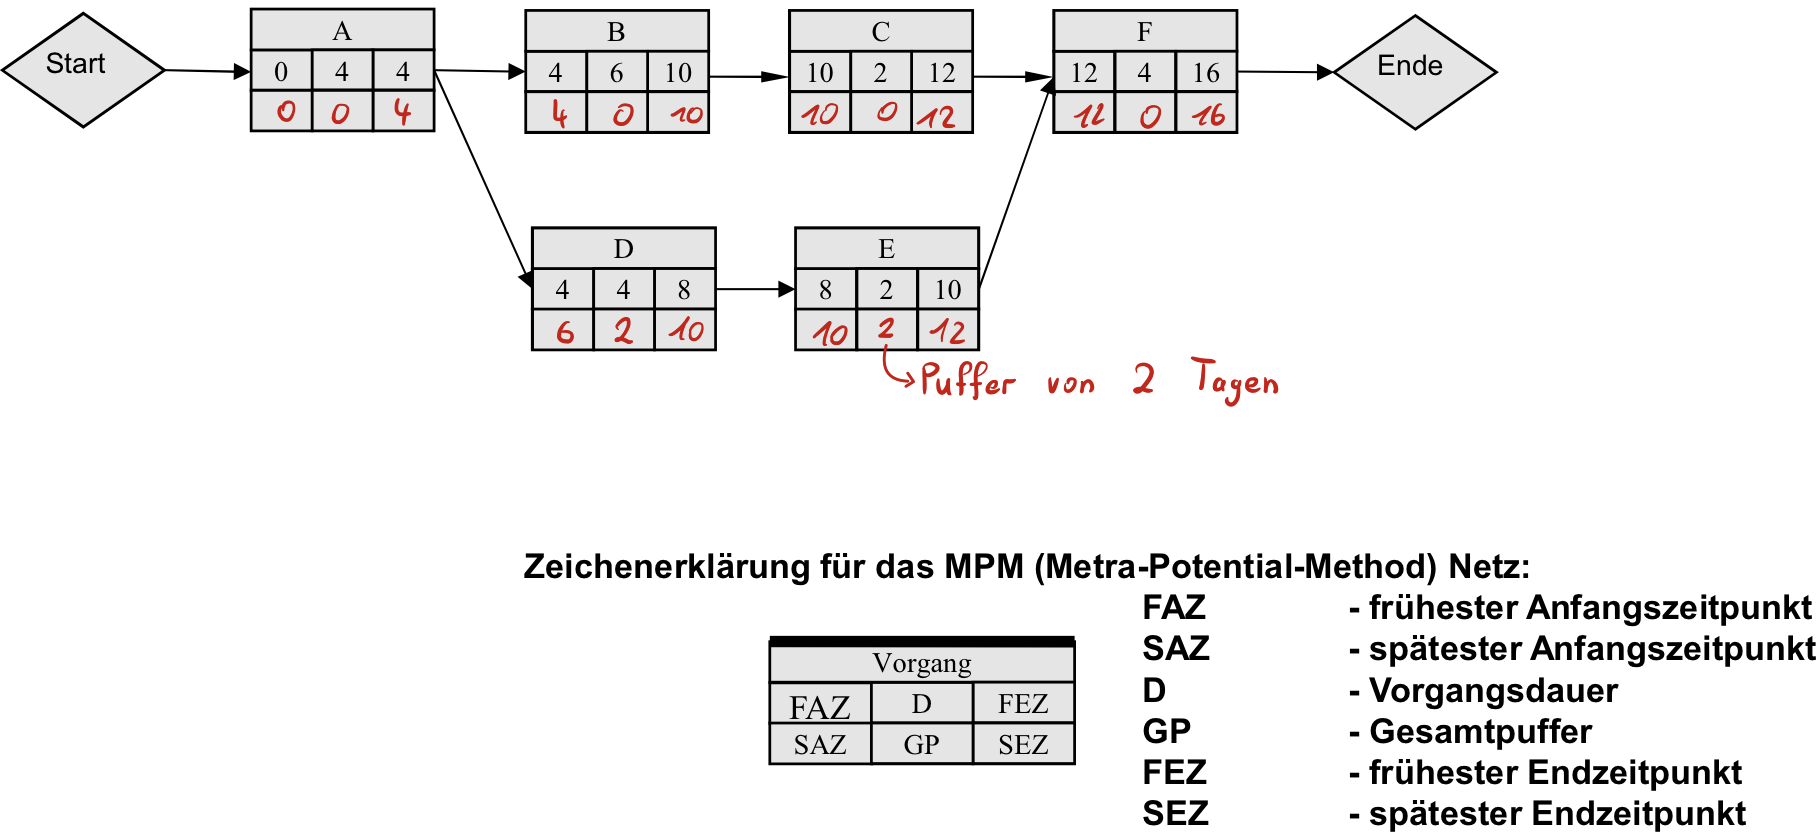
\includegraphics[scale=.175]{Bilder/MPM.JPG}	
	\end{center}
	\item Wie erhält man SEZ, SAZ und GP?
	\begin{enumerate}
		\item Durch das Rückwärtsrechnen (z.B. beim MPM-Plan)
	\end{enumerate}
	\item Was versteht man unter einer Normalfolge beim MPM und welche Folgen kennen sie noch?
	\begin{enumerate}
		\item Darunter versteht man \textcolor{red}{??} und außerdem gibts noch die Ende-Anfang-Folge
	\end{enumerate}
	\item Wozu dient der Kostenplan?
	\begin{enumerate}
		\item Frühzeitige Ermittlung der Kosten
		\item Preisermittlung für Auftraggeber
		\item Überwachung der Kosten
		\item Alternativfindung
	\end{enumerate}
	\item Weshalb ist eine gute Kostenschätzung bereits zum Beginn des Projektes wichtig?
	\begin{enumerate}
		\item Budgetbildung 
		\item Alternativen aufzeigen
	\end{enumerate}
	\item Wieso sollte man ein Projekt in verschiedene Phasen strukturieren?
	\begin{enumerate}
		\item Zwischenstände
		\item Entwicklungszyklen
		\item Transparenz/Übersichtlichkeit
		\item Strukturierung
	\end{enumerate}
	\item Beschreiben Sie die einzelnen Phasen eines Projektvorgehensmodell?
	\begin{enumerate}
		\item Definition
		\item Analyse
		\item Entwurf
		\item Implementierung
		\item Inbetriebnahme
	\end{enumerate}
	\item Was versteht man unter einem sequentiellen Vorgehensmodell?
	\begin{enumerate}
		\item Ein Schritt nach dem anderen
		\item Nach jedem Schritt erfolgt ein Ergebnis
	\end{enumerate}
	\item Was ist das besondere am Wasserfallmodell?
	\begin{enumerate}
		\item Rücksprünge in vorhergehende Phase möglich(bei Fehlern)
	\end{enumerate}
	\item Worin liegt die Weiterentwicklung des V-Modells gegenüber dem Wasserfallmodell?
	\begin{enumerate}
		\item Es werden Tests erstellt, welche die vorherigen Erzeugnisse und Anforderungen testen/überprüfen
		\item schränkt Freiheitsgrade ein, daher auch gut für größere Projekte
	\end{enumerate}
	\item Was bedeuted die Aussage: Phasenmodelle müssen zum Projekt passen?
	\begin{enumerate}
		\item Projekte sind individuell und benötigen unterschiedliche Phasenmodelle
		\item Man kann nicht für sämtliche Projekte immer das gleiche Phasenmodell nutzen, da andere besser passen würden und man je nach Projekt entscheiden muss
	\end{enumerate}
	\item Wozu dient die Risikoplanung?
	\begin{enumerate}
		\item Zur Vorbereitung
		\item Maßnahmen bereit haben
		\item Möglichen Problemen aus dem Weg gehen
		\item Probleme früher erkennen
	\end{enumerate}
	\item Welche Probleme können bei der Risikoplanung auftreten?
	\begin{enumerate}
		\item Risiken nicht erkennen
		\item Risiken unterschätzen
		\item Ausmaß falsch einschätzen
	\end{enumerate}
	\item Aus welchen Elementen besteht ein Risikokreislauf?
	\begin{enumerate}
		\item Risiken erkennen
		\item Risiken analysieren
		\item Maßnahmen planen 
		\item Maßnahmen umsetzen
		\item \textit{Repeat}
	\end{enumerate}
	\item Weshalb ist das Risikomanagement ein Prozess?
	\begin{enumerate}
		\item Weil feste Schritte regelmäßig ausgeführt werden
	\end{enumerate}
	\item Wie ermittelt man die Bedrohung durch ein Risiko?
	\begin{enumerate}
		\item Eintrittswahrscheinlichkeit $\cdot$ Kosten(Ausmaß)
	\end{enumerate}
	\item Wie und wo können Risiken in einem Projekt entdeckt werden?
	\begin{enumerate}
		\item Erfahrung
		\item Vertrag
		\item Gesetze
		\item Gremien \textcolor{red}{??}
	\end{enumerate}
	\item Wie kann mit den entdeckten Risiken verfahren werden?
	\begin{enumerate}
		\item Prävention
		\item Akzeptanz
		\item \textcolor{red}{??}
	\end{enumerate}
	\item Nennen Sie typische Risiken in einem IT-Projekt?
	\begin{enumerate}
		\item Hardware funktioniert nicht
		\item zu späte Lieferungen
		\item Stromausfälle
		\item Kapazität
		\item Richtlinien nicht eingehalten
	\end{enumerate}
	\item Was bedeuted \textit{agil} in der Softwareentwicklung?
	\begin{enumerate}
		\item Dynamisch auf Änderungen reagieren
		\item Probleme und Fehler erkennen und beheben/verbessern
	\end{enumerate}
	\item Wir sprechen von inkremetell und iterativ. Erklären Sie diese beiden Begriffe anhand des Vorgehensmodells von Scrum?
	\begin{enumerate}
		\item Inkrementell: Auf einander aufbauend
		\item Iterativ: Schrittweise sich wiederholender Prozess
	\end{enumerate}
	\item Welche Nachteile hat das Wasserfallmodell gegenüber der agilen Softwareentwicklung?
	\begin{enumerate}
		\item Unflexibel
		\item Starr 
		\item Schlecht im Nachhinein korrigierbar
		\item wird erst am Ende der Entwicklung dem Auftraggeber präsentiert
	\end{enumerate}
	\item Bei welcher Art von Projekten empfehlen Sie mir keine agile Methode?
	\begin{enumerate}
		\item Bei einfachen und übersichtlichen Projekten(kleine Projekte)
		\item Wenn die Technologie schon bekannt ist
	\end{enumerate}
	\item Welches sind die wesentlichen agilen Prinzipien?
	\begin{enumerate}
		\item Individuen und Interaktionen
		\item Funktionierende Software
		\item Zusammen mit dem Auftraggeber(ständige Absprache und Anpassung)
		\item Auf unbekannte Änderungen einstellen
	\end{enumerate}
	\item Ist Scrum eine PRM-Methode?
	\begin{enumerate}
		\item Nein, Scrum ist ein Vorgehensmodell
	\end{enumerate}
	\item Wozu dient das Product-Backlog?
	\begin{enumerate}
		\item Das Product-Backlog ist eine Sammlung an allen Aufgaben, die über das Projekt anfallen(Storys nicht unbedingt ausformuliert)
	\end{enumerate}
	\item Was ist der Unterschied zwischen einer Anforderungsbeschreibung und einer User-Story?
	\begin{enumerate}
		\item Anforderungsbeschreibung am Anfang schon recht genau
		\item Eine Story hingegen wird immer weiter spezifiziert
	\end{enumerate}
	\item Welche Rollen gibt es bei Scrum?
	\begin{enumerate}
		\item Scrum Master
		\item Team 
		\item Project Owner
	\end{enumerate}
	\item Welche Rollen spielt der Projektleiter bei Scrum?
	\begin{enumerate}
		\item Der Projektleiter existiert im klassischen Sinne nichtmehr und seine Aufgaben werden an die oben genannten Rollen verteilt
	\end{enumerate}
	\item Was sind die Aufgaben des Scrum Masters?
	\begin{enumerate}
		\item Dafür zu sorgen, dass keine Behinderungen auftreten und das Team in Ruhe arbeiten kann
		\item Sorgt dafür, dass die Scrum-Prozess ohne Probleme/Fehler laufen
	\end{enumerate}
	\item Was sind die Aufgaben des Product Owners?
	\begin{enumerate}
		\item Der Product Owner ist die Schnittstelle zum Auftraggeber(Kunde)
		\item Befüllt und schreibt das Product Backlog
	\end{enumerate}
	\item Wozu dient das Daily bei Scrum?
	\begin{enumerate}
		\item Gegenseitige Information
		\item Bekanntgabe von Behinderungen und Problemen
	\end{enumerate}
\end{enumerate}
\end{document}